\documentclass[aspectratio=43,serif]{beamer}
\setbeamersize{text margin left=5pt, text margin right=5pt, sidebar width left=0pt,sidebar width right=0pt}
\usepackage{tikz}
\usetikzlibrary{positioning}
\usetikzlibrary{fit}
\usetikzlibrary{shapes.geometric}
\usetikzlibrary{calc}
\usetikzlibrary{patterns}
\usetikzlibrary{decorations.pathreplacing}
\usetikzlibrary{decorations.markings}
\usetikzlibrary{arrows.meta}
\usepackage{pgfplots}
\usepackage{graphicx}
\usepackage{dcolumn}
\newcolumntype{d}[1]{D{.}{.}{#1}}
\usepackage{booktabs}
\usepackage{mathspec}
\setallmainfonts(Digits,Latin,Greek)[
	Ligatures={TeX,Common},
	Path=./fonts/,
	PunctuationSpace=0,							
	%Numbers={OldStyle,Proportional},				% for tables use \addfontfeatures{Numbers={Monospaced,Lining}}
	Numbers={Proportional},	% normal numbers			% for tables use \addfontfeatures{Numbers={Monospaced,Lining}}
	BoldFont = LinLibertine_RZ_B.otf ,				% semi-bold
	ItalicFont = LinLibertine_RI_B.otf ,			
	BoldItalicFont = LinLibertine_RZI_B.otf 		% semi-bold
	]{LinLibertine_R_B.otf}	
\usepackage{langsci/langsci-tbls}

%%%%%%%%%%%%%%%%%%%%%%%%%%%%%%%%%%%%%%%%%%%%%%%%%%%%%%%%%%%%%%%%%%%%%
%
%    Color definitions:
%
%%%%%%%%%%%%%%%%%%%%%%%%%%%%%%%%%%%%%%%%%%%%%%%%%%%%%%%%%%%%%%%%%%%%%

\definecolor{lsLightBlue}{cmyk}{0.6,0.05,0.05,0}
\definecolor{lsMidBlue}{cmyk}{0.75,0.15,0,0}
\definecolor{lsMidDarkBlue}{cmyk}{0.9,0.4,0.05,0}
\definecolor{lsDarkBlue}{cmyk}{0.9,0.5,0.15,0.3}
\definecolor{lsNightBlue}{cmyk}{1,0.47,0.22,0.68}
\definecolor{lsYellow}{cmyk}{0,0.25,1,0}
\definecolor{lsLightOrange}{cmyk}{0,0.50,1,0}
\definecolor{lsMidOrange}{cmyk}{0,0.64,1,0}
\definecolor{lsDarkOrange}{cmyk}{0,0.78,1,0}
\definecolor{lsRed}{cmyk}{0.05,1,0.8,0}
\definecolor{lsLightWine}{cmyk}{0.3,1,0.6,0}
\definecolor{lsMidWine}{cmyk}{0.54,1,0.65,0.1}
\definecolor{lsDarkWine}{cmyk}{0.58,1,0.70,0.35}
\definecolor{lsSoftGreen}{cmyk}{0.32,0.02,0.72,0}
\definecolor{lsLightGreen}{cmyk}{0.4,0,1,0}
\definecolor{lsMidGreen}{cmyk}{0.55,0,0.9,0.1}
\definecolor{lsRichGreen}{cmyk}{0.6,0,0.9,0.35}
\definecolor{lsDarkGreenOne}{cmyk}{0.85,0.02,0.95,0.38}
\definecolor{lsDarkGreenTwo}{cmyk}{0.85,0.05,1,0.5}
\definecolor{lsNightGreen}{cmyk}{0.88,0.15,1,0.66}
\definecolor{lsLightGray}{cmyk}{0,0,0,0.17}
\definecolor{lsGuidelinesGray}{cmyk}{0,0.04,0,0.45}
 
\definecolor{langscicol1}{cmyk}{0.6,0.05,0.05,0}
\definecolor{langscicol2}{cmyk}{0.75,0.15,0,0}
\definecolor{langscicol3}{cmyk}{0.9,0.4,0.05,0}
\definecolor{langscicol4}{cmyk}{0.9,0.5,0.15,0.3}
\definecolor{langscicol5}{cmyk}{1,0.47,0.22,0.68}
\definecolor{langscicol6}{cmyk}{0,0.25,1,0}
\definecolor{langscicol7}{cmyk}{0,0.50,1,0}
\definecolor{langscicol8}{cmyk}{0,0.64,1,0}
\definecolor{langscicol9}{cmyk}{0,0.78,1,0}
\definecolor{langscicol10}{cmyk}{0.05,1,0.8,0}
\definecolor{langscicol11}{cmyk}{0.3,1,0.6,0}
\definecolor{langscicol12}{cmyk}{0.54,1,0.65,0.1}
\definecolor{langscicol13}{cmyk}{0.58,1,0.70,0.35}
\definecolor{langscicol14}{cmyk}{0.32,0.02,0.72,0}
\definecolor{langscicol15}{cmyk}{0.4,0,1,0}
\definecolor{langscicol16}{cmyk}{0.55,0,0.9,0.1}
\definecolor{langscicol17}{cmyk}{0.6,0,0.9,0.35}
\definecolor{langscicol18}{cmyk}{0.85,0.02,0.95,0.38}
\definecolor{langscicol19}{cmyk}{0.85,0.05,1,0.5}
\definecolor{langscicol20}{cmyk}{0.88,0.15,1,0.66}


\newcommand{\lsptable}[2]{
\resizebox{#1}{!}{
\begin{tabularx}{\textwidth}{XXXXXXXXXXXXXXXXXXXX}
 \cellcolor{langscicol1}&\cellcolor{langscicol2}&\cellcolor{langscicol3}&\cellcolor{langscicol4}&\cellcolor{langscicol5}&\cellcolor{langscicol6}&\cellcolor{langscicol7}&\cellcolor{langscicol8}&\cellcolor{langscicol9}&\cellcolor{langscicol10}&\cellcolor{langscicol11}&\cellcolor{langscicol12}&\cellcolor{langscicol13}&\cellcolor{langscicol14}&\cellcolor{langscicol15}&\cellcolor{langscicol16}&\cellcolor{langscicol17}&\cellcolor{langscicol18}&\cellcolor{langscicol19}&\cellcolor{langscicol20}
 \rule{0pt}{#2}
\end{tabularx}
}
}

\begin{document}

\frame{{\tiny\sffamily (from Berghäll 2015)}
\begin{columns}[c]
\begin{column}{62mm}
 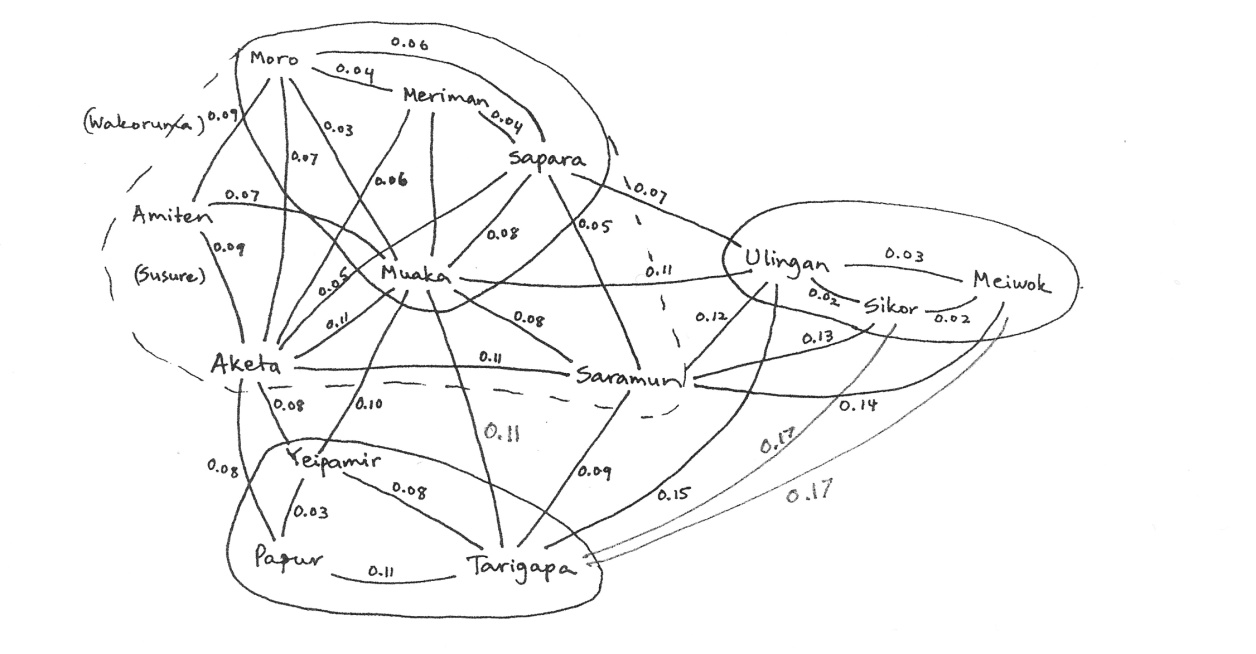
\includegraphics[width=\textwidth]{im/BerghallMeanDegrees.jpeg}
\end{column}
\hfill%
\begin{column}{62mm}
 \resizebox{\textwidth}{!}{\pgfdeclarelayer{bg}
\pgfdeclarelayer{bg2}
\pgfsetlayers{bg2,bg,main}
\resizebox{\textwidth}{!}{
\begin{tikzpicture}[baseline]


\node	(moro)				at	(0,0)									{Moro};
\node	(meriman)			[below right=9mm and 21mm of moro]			{Meriman};
\node	(sapara)			[below right=6mm and 12mm of meriman]		{Sapara};
\node	(muaka)				[below=20mm of meriman]						{Muaka};
\node	(amiten)			[below left=20mm and 13mm of moro]			{Amiten};	
\node	(aketa)				[below=45mm of moro]		{Aketa};
\node	(saramun)			[right=46.75mm of aketa]						{Saramun};
\node	(yeipamir)			[below right=9mm and 18mm of aketa]			{Yeipamir};
\node	(papur)				[below right=24mm and 0mm of aketa]			{Papur};
\node	(tarigapa)			[right=30mm of papur]						{Tarigapa};
\node	(ulingan)		  	[right=40mm of muaka]						{Ulingan};
\node	(meiwok)			[right=30mm of ulingan]						{Meiwok};
\node	(sikor)				[right=39mm of saramun]		{Sikor};

\node	(susure)			[below=15mm of amiten]						{(Susure)};
\node	(wakoruma)			[below left=8mm and 17mm of moro]			{(Wakoruma)};


% Categories
\begin{pgfonlayer}{bg}
\node (kat1) [fill=gray!15, draw, dashed, rounded corners=15, fit=(moro) (meriman) (sapara) (muaka)] {};
\node (kat2) [fill=gray!15, draw, dashed, rounded corners=15, fit= (ulingan) (sikor) (meiwok)] {};
\node (kat3) [fill=gray!15, draw, dashed, rounded corners=15, fit= (papur) (yeipamir) (tarigapa)] {}; 
\end{pgfonlayer}
\begin{pgfonlayer}{bg2}
\node (kat4) [fill=gray!5,draw, dotted, rounded corners=15, fit = (kat1) (amiten) (aketa) (saramun), inner sep=10pt]{}; 
\end{pgfonlayer}

\footnotesize{
% Moro Relations
\path	(moro)	edge node [sloped, above] {0.04}							(meriman);
\path (moro)	edge [bend left] node [sloped, above] {0.06}	(sapara);
\path (moro)	edge [bend right=10] node [sloped, above] {0.03} (muaka);
\path (moro) 	edge node [sloped, below] {0.07} (aketa);
\path (moro)	edge [bend right] node [sloped, above] {0.09} (amiten); 

% Meriman Relations
\path (meriman) 	edge [sloped, above] node {0.04} (sapara);
\path (meriman) 	edge node [sloped, above] {0.04} (aketa);
\path (meriman) 	edge node [sloped, above, pos=0.333] {0.07} (muaka);

% Sapara Relations
\path (sapara) 	edge [bend right=20] node [sloped, above right] {0.05} (aketa);
\path (sapara) 	edge node [sloped, above] {0.07} (ulingan);
\path (sapara) 	edge node [sloped, below left] {0.05} (saramun);
\path (sapara) 	edge node [sloped, above left] {0.08} (muaka);

% Amiten Relations
\path (amiten)	edge node [sloped, below] {0.07}	(muaka);
\path (amiten)	edge [bend right] node [sloped,below left] {0.09}	(aketa);

% Muaka Relations
\path (muaka)	edge node [sloped, above right] {0.11}	(ulingan);
\path (muaka)	edge node [sloped, below] {0.08}	(saramun);
\path (muaka)	edge node [sloped, above] {0.11}	(tarigapa);
\path (muaka)	edge [bend left=10] node [sloped, below, pos=0.575] {0.10}	(yeipamir);
\path (muaka)	edge node [sloped, below] {0.11}	(aketa);

% Ulingan Relations
\path (ulingan) edge node [sloped, below] {0.12}	(saramun);
\path (ulingan) edge node [sloped, above] {0.15}	(tarigapa);
\path (ulingan) edge node [sloped, above] {0.02}	(sikor);
\path (ulingan) edge node [sloped, above] {0.03}	(meiwok);

% Aketa Relations
\path (aketa) edge node [sloped, below, pos=0.333] {0.08}	(papur);
\path (aketa) edge node [sloped, above] {0.08}	(yeipamir);
\path (aketa) edge node [sloped, below] {0.11}	(saramun);

% Saramun Relations
\path (saramun) edge node [sloped, below] {0.09}	(tarigapa);
\path (saramun) edge [bend left=35] node [above, sloped] {0.14}	(meiwok);
\path (saramun) edge node [sloped, above] {0.13}	(sikor);

% Sikor Relations
\path (sikor) edge node [sloped, above] {0.02}	(meiwok);
\path (sikor) edge node [sloped, below right] {0.14}	(tarigapa);

% Meiwok Relations
\path (meiwok) edge [bend left] node [sloped, below right] {0.17}	(tarigapa);

% Yeipamir Relations
\path (yeipamir) edge node [sloped, above] {0.03} (papur);
\path (yeipamir) edge node [sloped, below] {0.08} (tarigapa);

% Papur Relations
\path (papur) edge node [below] {0.11} 	(tarigapa);

% Tarigapa Relations
% Will be empty for now.
}
\end{tikzpicture}
}}
\end{column}%
\end{columns}}

\frame{{\tiny\sffamily (from Berghäll 2015)}
\begin{columns}[c]
\begin{column}{62mm}
 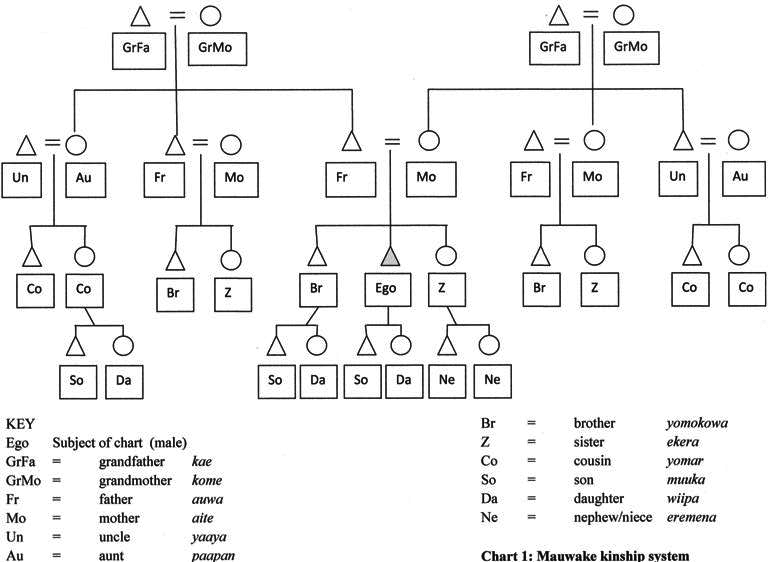
\includegraphics[width=\textwidth]{im/BeghallKinship.png}
\end{column}
\hfill%
\begin{column}{62mm}
 \resizebox{\textwidth}{!}{%1-mauwake_kinship_system_cart.tex
\resizebox{\textwidth}{!}{
\begin{tikzpicture}

%	Naming Convention for this Picture
%	-------------------------------------
%	Text nodes are in normal letters
%	Shape notes are in ALLCAPS
%
%	Nodes are named 1-n depending on the distance to Ego 
%	Those left of Ego are preceeded by n, those right of Ego are followed by their indexical n

%	Margin conventions
%	Horizontally: Within children of the same parents: 1cm
%		-"-		  Within children of diff. parents: 1.75cm
%
%	Vertically:   Within children of diff. parents: 3.5cm

%Padding for family members
[every rectangle node/.style={inner sep=6pt}]
%circle size, globally
% [every circle node/.sytle={minimum size=.6cm}] Doesn't work, why?

%Ego
\node at (0,0) [rectangle, draw] (ego) {Ego};
\node [above=.1cm of ego,regular polygon, regular polygon sides=3, draw, fill=gray] (EGO) {}; 
%Brother of Ego
\node [left=3cm of ego, rectangle, draw] (1br) {Br};
\node [above=.1cm of 1br, regular polygon, regular polygon sides=3, draw] (1BR) {};
%Sister of Ego
\node [right=3cm of ego, rectangle, draw] (z1) {Z};
\node [above=.1cm of z1, circle, minimum size=.6cm, draw] (Z1) {};

% Ego's cousins on their mother's side
\node [right=1.75cm of z1, rectangle, draw] (br1) {Br};
\node [above=.1cm of br1, regular polygon, regular polygon sides=3, draw] (BR1) {};
\node [right=1cm of br1, rectangle, draw] (z2) {Z};
\node [above=.1cm of z2, circle, minimum size=.6cm, draw] (Z2) {};

\node [right=1.75cm of z2, rectangle, draw] (co1) {Co};
\node [above=.1cm of co1, regular polygon, regular polygon sides=3, draw] (CO1) {};
\node [right=1cm of co1, rectangle, draw] (co2) {Co};
\node [above=.1cm of co2, circle, minimum size=.6cm, draw] (CO2) {};

% Ego's cousins on their mother's side
\node [left=1.75cm of 1br, rectangle, draw] (1z) {Z};
\node [above=.1cm of 1z, circle, minimum size=.6cm, draw] (1Z) {};
\node [left=1cm of 1z, rectangle, draw] (2br) {Br};
\node [above=.1cm of 2br, regular polygon, regular polygon sides=3, draw] (2BR) {};

\node [left=1.75cm of 2br, rectangle, draw] (1co) {Co};
\node [above=.1cm of 1co, circle, minimum size=.6cm, draw] (1CO) {};
\node [left=1cm of 1co, rectangle, draw] (2co) {Co};
\node [above=.1cm of 2co, regular polygon, regular polygon sides=3, draw] (2CO) {};

% Ego's parents
\node [above left=3.5cm and .5cm of ego, rectangle, draw] (1fr) {Fr};
\node [above=.1cm of 1fr, regular polygon, regular polygon sides=3, draw] (1FR) {};
\node [above right=3.5cm and .5cm of ego, rectangle, draw] (mo1) {Mo};
\node [above=.1cm of mo1, circle, minimum size=.6cm, draw] (MO1) {};

% Marriage smyol of Ego's parents
\node [above=3.5cm of EGO] (1frmo1) {\huge{=}};

% Ego's Aunties and Uncles
\node [above=3.5cm of br1, rectangle, draw] (fr1) {Fr};
\node [above=.1cm of fr1, regular polygon, regular polygon sides=3, draw] (FR1) {};
\node [right=1cm of fr1, rectangle, draw] (mo2) {Mo};
\node [above=.1cm of mo2, circle, minimum size=.6cm, draw] (MO2) {};
\node at ($(MO2) !.5! (FR1)$) (fr1mo2) {\huge{=}};

\node [above=3.5cm of co1, rectangle, draw] (un1) {Un};
\node [above=.1cm of un1, regular polygon, regular polygon sides=3, draw] (UN1) {};
\node [right=1cm of un1, rectangle, draw] (au1) {Au};
\node [above=.1cm of au1, circle, minimum size=.6cm, draw] (AU1) {};
\node at ($(UN1) !.5! (AU1)$) (un1au1) {\huge{=}};

\node [above=3.5cm of 2br, rectangle, draw] (2fr) {Fr};
\node [above=.1cm of 2fr, regular polygon, regular polygon sides=3, draw] (2FR) {};
\node [right=1cm of 2fr, rectangle, draw] (1mo) {Mo};
\node [above=.1cm of 1mo, circle, minimum size=.6cm, draw] (1MO) {};
\node at ($(2FR) !.5! (1MO)$) (2fr1mo) {\huge{=}};

\node [above=3.5cm of 2co, rectangle, draw] (1un) {Un};
\node [above=.1cm of 1un, regular polygon, regular polygon sides=3, draw] (1UN) {};
\node [right=1cm of 1un, rectangle, draw] (1au) {Au};
\node [above=.1cm of 1au, circle, minimum size=.6cm, draw] (1AU) {};
\node at ($(1UN) !.5! (1AU)$) (1un1au) {\huge{=}};

% Ego's Grandparents
% ... on their father's side
\node [above=3.5cm of 2fr, rectangle, draw] (1grfa) {GrFa};
\node [above=.1cm of 1grfa, regular polygon, regular polygon sides=3, draw] (1GRFA) {};
\node [right=1cm of 1grfa, rectangle, draw] (1grmo) {GrMo};
\node [above=.1cm of 1grmo, circle, minimum size=.6cm, draw] (1GRMO) {};
\node at ($(1GRFA) !.5! (1GRMO)$) (1grfa1grmo) {\huge{=}};

% ... on their mother's side
\node [above=3.5cm of fr1, rectangle, draw] (grfa1) {GrFa};
\node [above=.1cm of grfa1, regular polygon, regular polygon sides=3, draw] (GRFA1) {};
\node [right=1cm of grfa1, rectangle, draw] (grmo1) {GrMo};
\node [above=.1cm of grmo1, circle, minimum size=.6cm, draw] (GRMO1) {};
\node at ($(GRFA1) !.5! (GRMO1)$) (grfa1grmo1) {\huge{=}};

% Ego's children
\node [below left=3.5cm and .5cm of ego, regular polygon, regular polygon sides=3, draw] (1SO) {};
\node [below=.1cm of 1SO, rectangle, draw] (1so) {So};
\node [right=1cm of 1so, rectangle, draw] (da1) {Da};
\node [above=.1cm of da1, circle, minimum size=.6cm, draw] (DA1) {};

% Ego's Nephews and Niece
\node [left=1.75cm of 1so, rectangle, draw] (1da) {Da};
\node [above=.1cm of 1da, circle, minimum size=.6cm, draw] (1DA) {};
\node [left=1cm of 1da, rectangle, draw] (2so) {So};
\node [above=.1cm of 2so, regular polygon, regular polygon sides=3, draw] (2SO) {};

\node [right=1.75cm of da1, rectangle, draw] (ne1) {Ne};
\node [above=.1cm of ne1, regular polygon, regular polygon sides=3, draw] (NE1) {};
\node [right=1cm of ne1, rectangle, draw] (ne2) {Ne};
\node [above=.1cm of ne2, circle, minimum size=.6cm, draw] (NE2) {};

% Ego's female Cousin's children 

\node [below left=3.5cm and .5cm of 1co, regular polygon, regular polygon sides=3, draw] (3SO) {};
\node [below=.1cm of 3SO, rectangle, draw] (3so) {So};
\node [right=1cm of 3so, rectangle, draw] (2da) {Da};
\node [above=.1cm of 2da, circle, minimum size=.6cm, draw] (2DA) {};


% In-Generation Connections

% Usage of in-generation connections:
% We are using Node Coordinate System, see Section 13.2.3 of the PGF manual
% \draw (node cs:name=NAME, anchor=north) |- +(0,.5) -| (node cs:name=2ndNAME);
% note: We use anchor=north in order to prevent PGF from choosing any other, just in case. We will probably not need it in the second node, though
% note 2: +(0,.5) is a relative position, meaning .5 vertical positive change
% |- means: Go vertical first and then horizontally

% Ego & their immediate Br & Z
\draw (node cs:name=EGO, anchor=north) |- +(0,.5) -| (node cs:name=Z1);
\draw (node cs:name=EGO, anchor=north) |- +(0,.5) -| (node cs:name=1BR);

% Ego's cousins on their mother's side
\draw (node cs:name=BR1, anchor=north) |- +(0,.5) -| (node cs:name=Z2) node [pos=.25] (MBR1Z2) {};
\draw (node cs:name=CO1, anchor=north) |- +(0,.5) -| (node cs:name=CO2) node [pos=.25] (MCO1CO2) {};

% Ego's cousins on their father's side
\draw (node cs:name=1Z, anchor=north) |- +(0,.5) -| (node cs:name=2BR) node [pos=.25] (M1Z2BR) {};
\draw (node cs:name=1CO, anchor=north) |- +(0,.5) -| (node cs:name=2CO) node [pos=.25] (M1CO2CO) {};

% Ego's fathers and his brother and sister
\draw (node cs:name=1FR, anchor=north) |- +(0,.5) -| (node cs:name=1AU);
\draw (node cs:name=1FR, anchor=north) |- +(0,.5) -| (node cs:name=2FR) node [pos=.25] (M1FR2FR) {};

% Ego's mother and her brother and sister
\draw (node cs:name=UN1, anchor=north) |- +(0,.5) -| (node cs:name=MO2);
\draw (node cs:name=UN1, anchor=north) |- +(0,.5) -| (node cs:name=MO1) node [pos=.25] (MUN1NO1) {};

% Ego's children and nephews/nieces
\draw (node cs:name=1SO, anchor=north) |- +(0,.5) -| (node cs:name=DA1) node [pos=.25] (M1SODA1) {};
\draw (node cs:name=NE1, anchor=north) |- +(0,.5) -| (node cs:name=NE2) node [pos=.25] (MNE1NE2) {}; % relative positioning. Not sure why it's 1/4, tough. 
\draw (node cs:name=2SO, anchor=north) |- +(0,.5) -| (node cs:name=1DA) node [pos=.25] (M2SO1DA) {};
\draw (node cs:name=3SO, anchor=north) |- +(0,.5) -| (node cs:name=2DA) node [pos=.25] (M3SO2DA) {};


% Between-Generation Connections

% The old way was \draw (node cs:name=grfa1grmo1, anchor=south) -- ($(grfa1grmo1)-(0,3.225)$); This was extremly messy.
% The new way is to use |- and a seperate node on the |--| specified above. A little tricky, but it should be reliable.


\draw (node cs:name=1frmo1, anchor=south) -- (node cs:name=EGO, anchor=north);
\draw (node cs:name=fr1mo2, anchor=south) |- (node cs:name=MBR1Z2, anchor=center);
\draw (node cs:name=un1au1, anchor=south) |- (node cs:name=MCO1CO2, anchor=center);
\draw (node cs:name=2fr1mo, anchor=south) |- (node cs:name=M1Z2BR, anchor=center);
\draw (node cs:name=1un1au, anchor=south) |- (node cs:name=M1CO2CO, anchor=center);
\draw (node cs:name=grfa1grmo1, anchor=south) |- (node cs:name=MUN1NO1, anchor=center);
\draw (node cs:name=1grfa1grmo, anchor=south) |- (node cs:name=M1FR2FR, anchor=center);
\draw (node cs:name=1co, anchor=south) |- (node cs:name=M3SO2DA, anchor=center);
\draw (node cs:name=ego, anchor=south) |- (node cs:name=M1SODA1, anchor=center);

\draw (node cs:name=1br, anchor=south) |- (node cs:name=M2SO1DA, anchor=center); %This is precise
\draw (node cs:name=z1, anchor=south) |- (node cs:name=MNE1NE2, anchor=center); %This is precise


\end{tikzpicture}}

% \vspace{\baselineskip}
% 
% \begin{centering}
% \begin{tabular}{llllll}
% 	
% 	
% 	\toprule\toprule
% 	
% 	Ego 	& \multicolumn{2}{l}{Subject of chart (male)} &&& 		\\		
% 	GrFa	& grandfather	& {\itshape kae} & 	Br &	brother 	& {\itshape yomokowa}\\
% 	GrMo	& grandmother	& {\itshape kome} &	Z &		sister		& {\itshape ekera}\\
% 	Fr		&	father		& {\itshape auwa} &	Co &	cousin		& {\itshape yomar}\\
% 	Mo		&	mother		& {\itshape aite} &	So &	son			& {\itshape muuka}\\
% 	Un		&	uncle		& {\itshape yaaya} & Da &	daughter	& {\itshape wiipa}\\
% 	Au		&	aunt		& {\itshape paapan} & Ne &	nephew/nice & {\itshape eremena}\\
% 	
% 	\bottomrule\bottomrule
% 	
% \end{tabular}
% \end{centering}}
\end{column}%
\end{columns}}

\begin{frame}{\tiny\sffamily (from Fantinuoli et al (ed) 2015)}
\begin{columns}[T] % align columns
\begin{column}{60mm}
\centering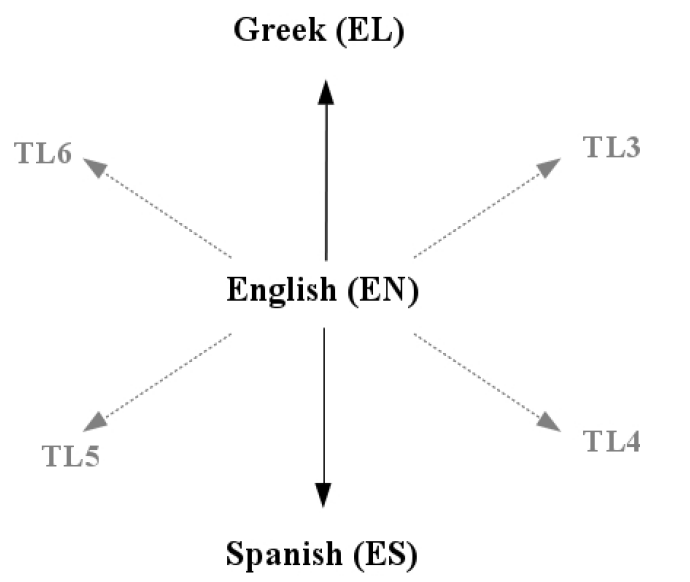
\includegraphics[width=.5\textwidth]{im/Fan-4-1.png}\\\vspace{2em}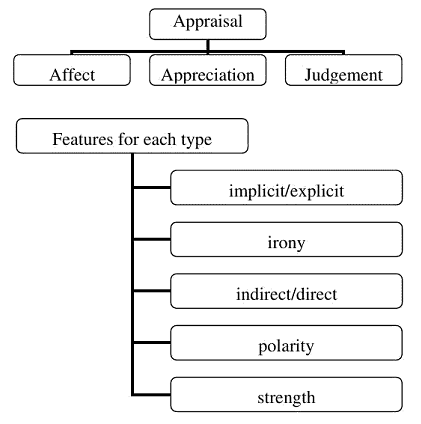
\includegraphics[width=.5\textwidth]{im/Fan-4-3.png}
\end{column}%
\hfill%
\begin{column}{60mm}
\centering\resizebox{.45\textwidth}{!}{	\begin{tikzpicture}
	
	\node at (0,0) (EN) {English (EN)};
	\node [below=2cm of EN] (ES) {Spanish (ES)};
	\node [above=2cm of EN] (EL) {Greek (EL)};
	
	\node [above left=1cm and 1cm of EN, color=gray] (TL6) {TL6};
	\node [above right=1cm and 1cm of EN, color=gray] (TL3) {TL3};
	\node [below left=1cm and 1cm of EN, color=gray] (TL5) {TL5};
	\node [below right=1cm and 1cm of EN, color=gray] (TL4) {TL4};
	
	\draw [ultra thick, -{Triangle[]}] (node cs:name=EN, anchor=north) -- (node cs:name=EL, anchor=south);
	\draw [ultra thick, -{Triangle[]}] (EN.south) -- (ES.north);
	
	\draw [thick, gray, dotted, -{Triangle[]}] (EN.south west) -- (TL5.north east);
	\draw [thick, gray, dotted, -{Triangle[]}] (EN.north west) -- (TL6.south east);
	\draw [thick, gray, dotted, -{Triangle[]}] (EN.north east) -- (TL3.south west);
	\draw [thick, gray, dotted, -{Triangle[]}] (EN.south east) -- (TL4.north west);
	
	\end{tikzpicture}}\\\vspace{2em}\resizebox{.55\textwidth}{!}{%4-3-Corpus-Annotation-Scheme.tex
\begin{tikzpicture}
[every rectangle node/.style={inner sep=6pt, rounded corners=5, draw}]


\node at (0,0) [rectangle] (appraisal) {Appraisal};
\node [below=5mm of appraisal, rectangle] (appreciation) {Appreciation};
\node [right=20mm of appreciation.east, rectangle] (judgement) {Jugdement};
\node [left=20mm of appreciation.west, rectangle] (affect) {Affect};

\draw [thick] (node cs:name=appraisal, anchor=south) -| (node cs:name=appreciation);
\draw [thick] (node cs:name=affect, anchor=north) |- +(0,.275) -| (node cs:name=judgement);


\node [below right=10mm and 0mm of affect.west, rectangle, text width=40mm, align=center] (features) {Features for each type}; 
\node [below right=4mm and 10mm of features.south, rectangle, text width=40mm, align=center] (implicit) {implicit/explicit};
\node [below=4mm of implicit, rectangle, text width=40mm, align=center] (irony) {irony};
\node [below=4mm of irony, rectangle, text width=40mm, align=center] (indirect) {indirect/direct};
\node [below=4mm of indirect, rectangle, text width=40mm, align=center] (polarity) {polarity};
\node [below=4mm of polarity, rectangle, text width=40mm, align=center] (strength) {strength};

\draw [thick] (node cs:name=features, anchor=south) |- (node cs:name=implicit);
\draw [thick] (node cs:name=features, anchor=south) |- (node cs:name=irony);
\draw [thick] (node cs:name=features, anchor=south) |- (node cs:name=indirect);
\draw [thick] (node cs:name=features, anchor=south) |- (node cs:name=polarity);
\draw [thick] (node cs:name=features, anchor=south) |- (node cs:name=strength);

\end{tikzpicture}}
\end{column}%
\end{columns}
\end{frame}


\begin{frame}{\tiny\sffamily (from Payne et al (ed) 2016)}
\begin{columns}[c] % align columns
\begin{column}{60mm}
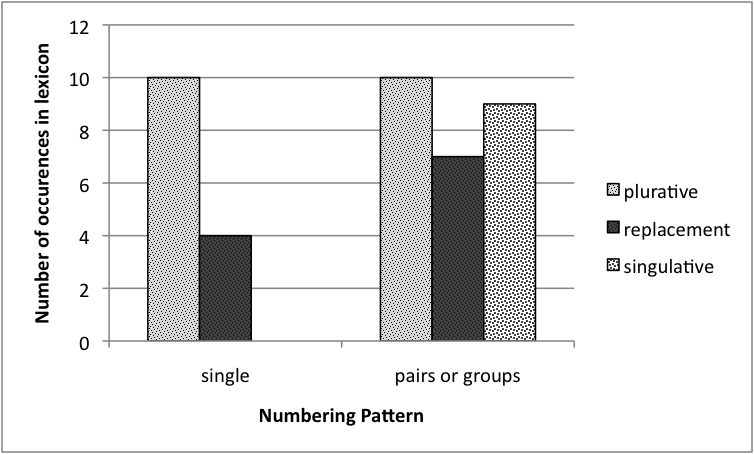
\includegraphics[width=\textwidth]{im/moodie-fig-2.png}
\end{column}%
\hfill%
\begin{column}{40mm}
\resizebox{\linewidth}{!}{\begin{tikzpicture}[trim axis left, trim axis right]
		\begin{axis}[ybar=0pt, ylabel={Number of occurences in lexicon}, xlabel={Numbering pattern},symbolic x coords={single, pairs or groups}, xtick=data, xtick align=center, bar width=2em, ymin=0, nodes near coords, nodes near coords align=vertical, xlabel near ticks, ymajorgrids, area legend, enlarge y limits={abs=2, upper}, enlarge x limits=0.5, legend entries={plurative,replacement,singuative}, legend style={cells={anchor=west}, legend pos=south east}]
		\addplot[pattern=dots] coordinates {(single,10)(pairs or groups,10)};
		\addplot[pattern=crosshatch] coordinates {(single,4)(pairs or groups,7)};
		\addplot[pattern=horizontal lines] coordinates {(single,0)(pairs or groups,9)};
		\end{axis}
		\end{tikzpicture}}
\end{column}%
\end{columns}
\end{frame}

\frame{{\tiny\sffamily (inspired by Drager 2015)}\fboxsep=0pt
\noindent%
\begin{minipage}[t]{0.48\linewidth}
\begin{table}[htbp]
\begin{center}
\resizebox{60mm}{!}{
\begin{tabular}{|l|r|r|r|}
   \hline
   feature & CR girl &  NCR girl & CR and NCR \\
   questions comparing & quote$-$dp &  quote$-$dp &  quote$-$dp \\
  \hline
  total number subjects & 23 & 19 & 42 \\
  total questions answered & 916 & 774 & 1690 \\
  total 1st token labeled as quote & 465 & 383 & 848 \\
  quote first on sheet & 278 & 231 &  509 \\
  1st token's context more likely & 110 & 73 &  183 \\
  1st and 2nd tokens' context matched & 271 & 242 & 513 \\
  1st token's context less likely & 84 & 68 & 152 \\
  1st token mean EucD & 1.5930 & 1.5400  & 1.5690 \\
  2nd token mean EucD & 1.6180 & 1.6720 & 1.6430 \\
  mean EucD diff. (Bark) & -0.02538  & -0.13280 &  -0.07388 \\
  1st token mean nuc F2 (Bark) & 11.25  & 11.19 & 11.23 \\
  2nd token mean nuc F2 (Bark) & 11.49 & 11.45 & 11.47 \\
  mean nuc F2 diff. (Bark) & -0.2379 & -0.2554  & -0.2458 \\
 	1st token mean duration ratio & 0.33900  & 0.32670 & 0.33350 \\
 	2nd token mean duration ratio & 0.35020  & 0.34520  & 0.34790 \\
  mean duration ratio diff. & -0.01120  & -0.01844 &  -0.01447 \\
  1st token $[$k$]$ present, 2nd token $[$k$]$ absent & 93  & 84  & 177\\
  1st token $[$k$]$ absent, 2nd token $[$k$]$ present & 74  & 65  & 139 \\
  $[$k$]$ present for both tokens & 118 & 83 & 201 \\
  $[$k$]$ absent for both tokens & 180  & 151 & 331 \\
    \hline
    
  
  \end{tabular}
}
% \caption{Charcteristics of quote$-$dp questions in Experiment 1 where the first token was identified as the quotative, by whether the participant was in a CR or a NCR group.}\label{tab:percExp1responsesqd2}
\end{center}
\end{table}\end{minipage}%
\hfill%
\begin{minipage}[t]{0.48\linewidth}
\begin{table}[htbp]
\begin{center}
\resizebox{60mm}{!}{
\begin{tabular}{ld{5}d{5}d{5}}
   \toprule\toprule
    & \multicolumn{3}{c}{features} \\\cmidrule(lr){2-4} 
   questions comparing quote$-$dp& \multicolumn{1}{c}{CR girl} &  \multicolumn{1}{c}{NCR girl} & \multicolumn{1}{c}{CR and NCR} \\
  \midrule
  total number subjects & 23 & 19 & 42 \\
  total questions answered & 916 & 774 & 1690 \\
  total 1st token labeled as quote & 465 & 383 & 848 \\
  quote first on sheet & 278 & 231 &  509 \\
  1st token's context more likely & 110 & 73 &  183 \\
  1st and 2nd tokens' context matched & 271 & 242 & 513 \\
  1st token's context less likely & 84 & 68 & 152 \\
  1st token mean EucD & 1.5930 & 1.5400  & 1.5690 \\
  2nd token mean EucD & 1.6180 & 1.6720 & 1.6430 \\
  mean EucD diff. (Bark) & -0.02538  & -0.13280 &  -0.07388 \\
  1st token mean nuc F2 (Bark) & 11.25  & 11.19 & 11.23 \\
  2nd token mean nuc F2 (Bark) & 11.49 & 11.45 & 11.47 \\
  mean nuc F2 diff. (Bark) & -0.2379 & -0.2554  & -0.2458 \\
 	1st token mean duration ratio & 0.33900  & 0.32670 & 0.33350 \\
 	2nd token mean duration ratio & 0.35020  & 0.34520  & 0.34790 \\
  mean duration ratio diff. & -0.01120  & -0.01844 &  -0.01447 \\
  1st token $[$k$]$ present, 2nd token $[$k$]$ absent & 93  & 84  & 177\\
  1st token $[$k$]$ absent, 2nd token $[$k$]$ present & 74  & 65  & 139 \\
  $[$k$]$ present for both tokens & 118 & 83 & 201 \\
  $[$k$]$ absent for both tokens & 180  & 151 & 331 \\
    \bottomrule
\bottomrule    
  
  \end{tabular}
}
% \caption{Characteristics of quote$-$dp questions in Experiment 1 where the first token was identified as the quotative, by whether the participant was in a CR or a NCR group.}\label{tab:percExp1responsesqd}
\end{center}
\end{table}\end{minipage}%
}

\begin{frame}{\tiny\sffamily (from Friesen 2016)}
\begin{columns}[c] % align columns
\begin{column}{60mm}
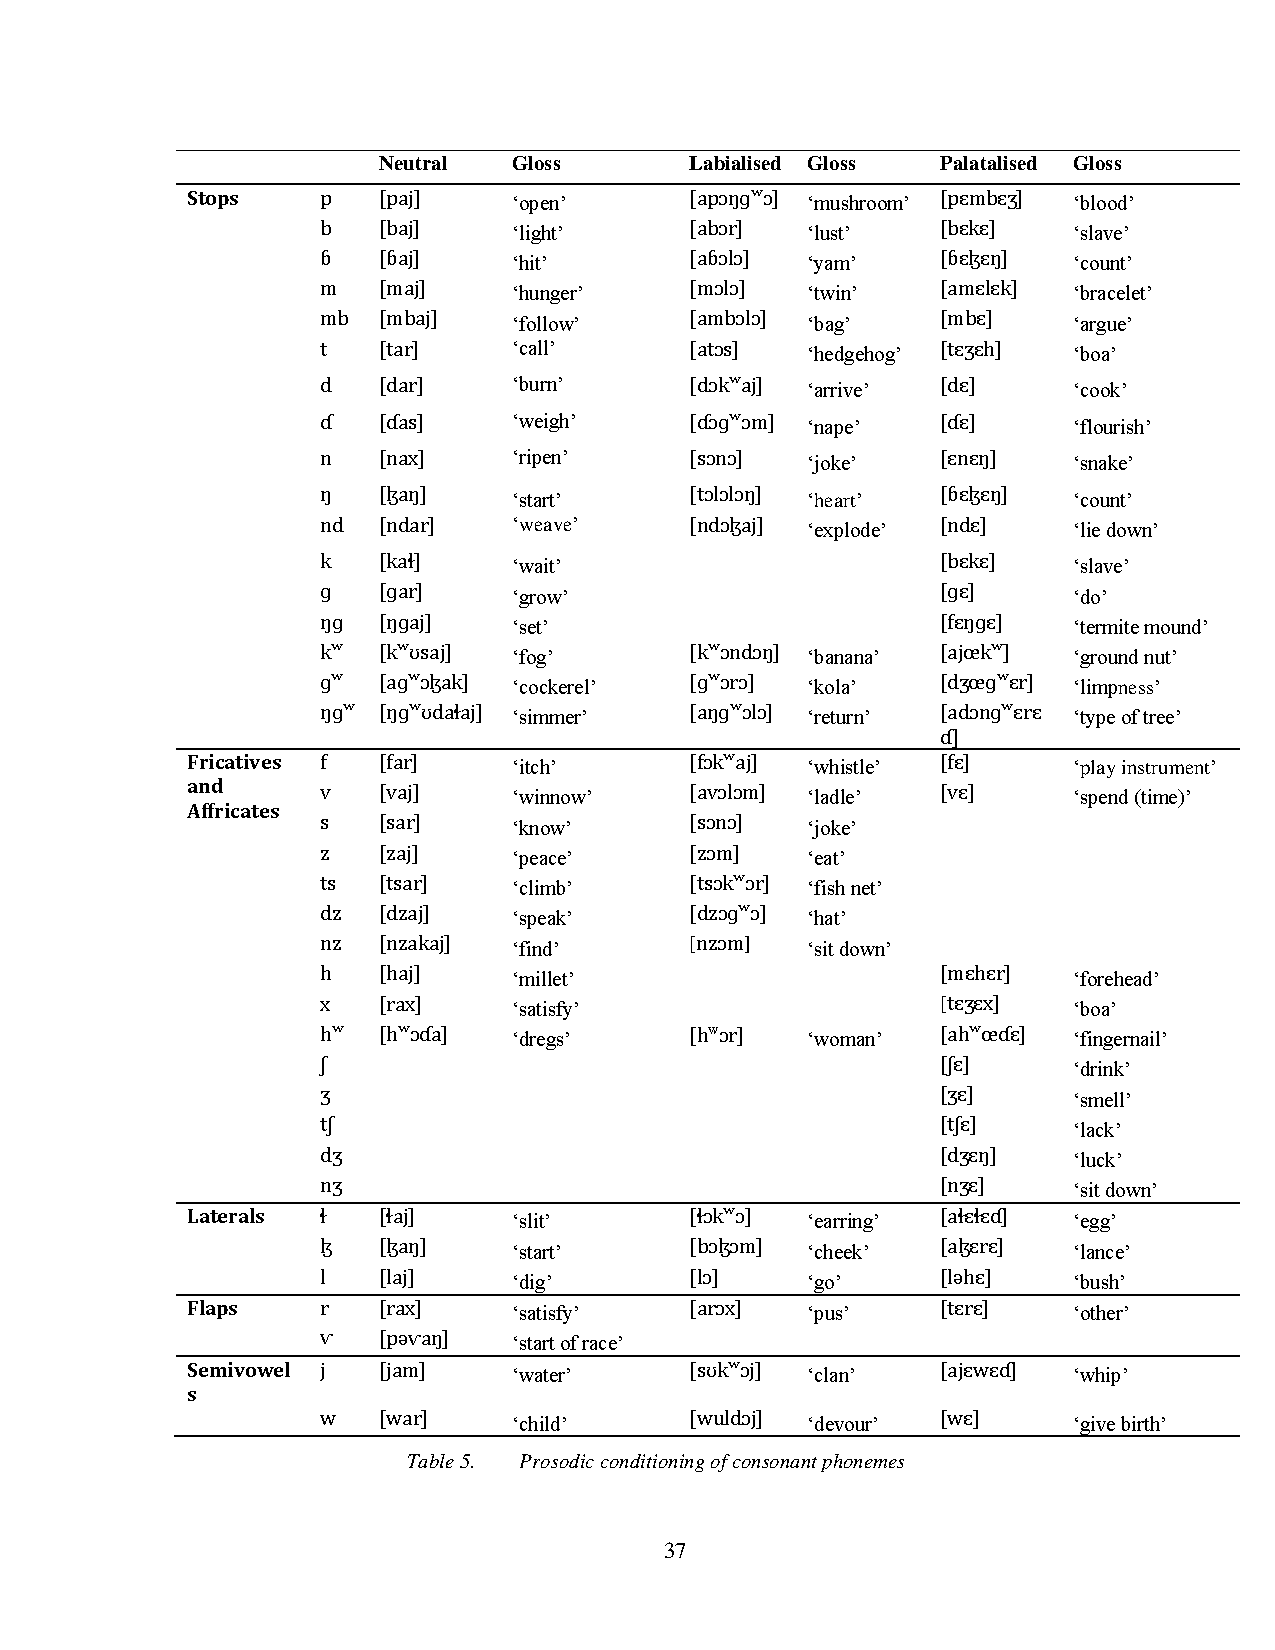
\includegraphics[width=\textwidth]{im/Moloko-Table5.pdf}
\end{column}%
\hfill%
\begin{column}{60mm}
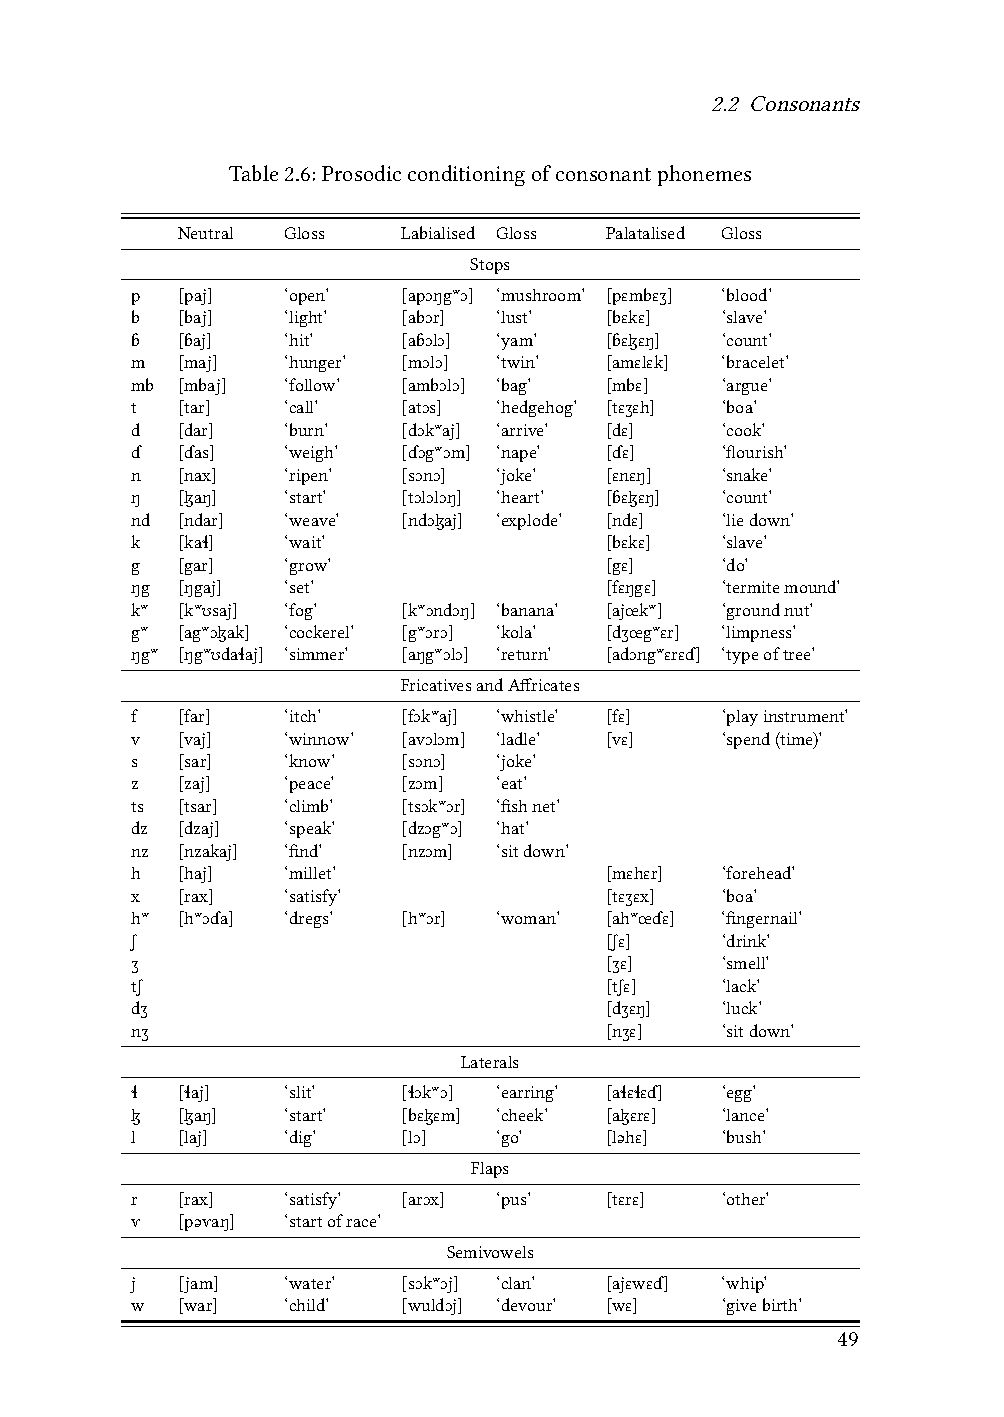
\includegraphics[width=\textwidth]{im/Moloko-new.pdf}
\end{column}%
\end{columns}
\end{frame}

\begin{frame}{\tiny\sffamily (inspired by Schäfer 2016)}\footnotesize
\tblsfr[lsYellow]{law}{Kompositionalität}{Die Bedeutung komplexer sprachlicher Ausdrücke ergibt sich aus der Be-
deutung ihrer Teile und der Art ihrer grammatischen Kombination. Diese
Eigenschaft von Sprache nennt man \emph{Kompositionalität}.}
\tblsfi{Weiterführende Literatur}{Eine sehr ausführliche Einführung in die artikulatorische Phonetik
ist Laver (1994). Einführende Darstellungen der deutschen Phonetik finden sich
z. B. in Rues u. a. (2009) und Wiese (2010).}
\end{frame}


\end{document}